\documentclass[12pt, letter]{article}
\usepackage{amsmath}
\usepackage{amssymb}
\usepackage{latexsym}
\usepackage{graphicx}
\usepackage[margin=2.5cm]{geometry}
\usepackage{setspace}
\usepackage{ctable}
\usepackage{booktabs}
\usepackage{caption}
\usepackage{subcaption}
\usepackage{siunitx}
\usepackage{enumitem}
\usepackage{multirow}
\usepackage{float}
\usepackage{hhline}
\usepackage{tabulary}
\usepackage[nottoc, notlof, notlot]{tocbibind}
\usepackage[framed]{mcode}
%\usepackage{indentfirst}
\usepackage{standalone}
\usepackage{fancyhdr}
\usepackage{array}
\newcolumntype{P}[1]{>{\raggedright\arraybackslash}p{#1}}
\lstset{breaklines}
\usepackage[hyphens]{url}
\usepackage{cleveref}
\setlength{\parindent}{0em}
%\renewcommand{\baselinestretch}{1.3}

\pagestyle{fancy}
\fancyhf{}
\lhead{SRK}
\rhead{Concept of Operations}

\begin{document}
%%%%%%%%%%%%%%%%%%%%%%%%%%%%%%%%%%%%%%%%%
% University Assignment Title Page 
% LaTeX Template
% Version 1.0 (27/12/12)
%
% This template has been downloaded from:
% http://www.LaTeXTemplates.com
%
% Original author:
% WikiBooks (http://en.wikibooks.org/wiki/LaTeX/Title_Creation)
%
% License:
% CC BY-NC-SA 3.0 (http://creativecommons.org/licenses/by-nc-sa/3.0/)
% 
% Instructions for using this template:
% This title page is capable of being compiled as is. This is not useful for 
% including it in another document. To do this, you have two options: 
%
% 1) Copy/paste everything between \begin{document} and \end{document} 
% starting at \begin{titlepage} and paste this into another LaTeX file where you 
% want your title page.
% OR
% 2) Remove everything outside the \begin{titlepage} and \end{titlepage} and 
% move this file to the same directory as the LaTeX file you wish to add it to. 
% Then add \input{./title_page_1.tex} to your LaTeX file where you want your
% title page.
%
%%%%%%%%%%%%%%%%%%%%%%%%%%%%%%%%%%%%%%%%%

%----------------------------------------------------------------------------------------
%	PACKAGES AND OTHER DOCUMENT CONFIGURATIONS
%----------------------------------------------------------------------------------------

\documentclass[12pt]{article}
\usepackage[margin=2.5cm]{geometry}

\begin{document}

\newcommand{\HRule}{\rule{\linewidth}{0.5mm}} % Defines a new command for the horizontal lines, change thickness here
\begin{titlepage}


\center % Center everything on the page
 
%----------------------------------------------------------------------------------------
%	HEADING SECTIONS
%----------------------------------------------------------------------------------------

\textsc{\LARGE University of Toronto}\\[1.2cm] % Name of your university/college
\textsc{\Large AER407 - Space Systems Design}\\[0.5cm] % Major heading such as course name
\textsc{\large Space Robo Korporation}\\[0.5cm] % Minor heading such as course title

%----------------------------------------------------------------------------------------
%	TITLE SECTION
%----------------------------------------------------------------------------------------

\HRule \\[0.4cm]
{ \huge \bfseries Concept of Operations for Canada's Next Generation Robotics}\\[0.5cm] % Title of your document
\HRule \\[1.2cm]

%----------------------------------------------------------------------------------------
%	LOGO SECTION
%----------------------------------------------------------------------------------------


\includegraphics[width=0.4\textwidth]{logo}\\[1cm] 

%----------------------------------------------------------------------------------------
%	AUTHOR SECTION
%----------------------------------------------------------------------------------------


\begin{centering} \large
\begin{tabular}{ll}
Operations	&	Guanchu Liu (999183011)	\\
Systems	&	Lian Liu (998700892)		\\
Mechanical	&	Jai Bansal (999856179)	\\
Electrical	& 	Hao Xing (999261345)	\\
Controls	&	Yun-Jae Kim (999870947)	\\[1cm]
\end{tabular}
\end{centering}


% If you don't want a supervisor, uncomment the two lines below and remove the section above
%\Large \emph{Author:}\\
%John \textsc{Smith}\\[3cm] % Your name

%----------------------------------------------------------------------------------------
%	DATE SECTION
%----------------------------------------------------------------------------------------

{\large \today}\\[3cm] % Date, change the \today to a set date if you want to be precise
 
%----------------------------------------------------------------------------------------

\vfill % Fill the rest of the page with whitespace

\end{titlepage}
\end{document}		%Cover page
\cfoot{\normalsize\thepage}
\pagenumbering{roman}% Roman-numbered pages (start from i)
\onehalfspacing
\newpage
\begin{document}
\topskip0pt
\vspace*{\fill}
\begin{center}
\large
\textbf{Executive Summary}
\end{center}

\normalsize
The following document outlines the operations involved in the mission to assist the development of a future lunar Outpost. After a description of the background, objectives, and scope of the mission, some of the key trade-offs in the mission are discussed, including its capability, level of autonomy, and mobility. Next, operational policies, constraints, environment and risk factors are defined, followed by a list of performance characteristics and quality attributes that can be used to judge the design of the system. A list of the different modes of operation, and user classes associated with the system is stated. Lastly, a series of flow diagrams are illustrated to provide some detailed information on the system's various interfaces with other systems, users, and interfaces under certain circumstances. 

\vspace*{\fill}

\end{document}
\newpage
\tableofcontents
\newpage
\listoffigures
\listoftables
\newpage
\begin{document}

\section*{List of Symbols}

\normalsize
\begin{tabular}{ll}
\textbf{ARM}	&	Asteroid Retrieval Mission	\\
\textbf{CC}	&	Customer Constraints	\\
\textbf{CSA}	&	Canadian Space Agency	\\
\textbf{EMI}	&	Electromagnetic Interference	\\
\textbf{EML2}	&	Earth-Moon Lagrange Point 2	\\
\textbf{ESA}	&	European Space Agency	\\
\textbf{EVA}	&	Extravehicular Activity	\\
\textbf{GC}	&	Government Constraints	\\
\textbf{ISECG}	&	International Space Exploration Consultation Group	\\
\textbf{ISO}	&	International Organization for Standardization	\\
\textbf{ISS}	&	International Space Station	\\
\textbf{JAXA}	&	Japanese Aerospace Exploration Agency	\\
\textbf{LEO}	&	Low Earth Orbit	\\
\textbf{LOS}	&	Loss of Signal	\\
\textbf{MDA}	&	MacDonald, Dettwiler and Associates Ltd.	\\
\textbf{MPCV}	&	Multi-Purpose Crew Vehicle	\\
\textbf{NASA}	&	National Aeronautics and Space Administration	\\
\textbf{RFP}	&	Request for Proposal	\\
\textbf{RSA}	&	Russian Space Agency	\\
\textbf{TBC}	&	To be confirmed	\\
\textbf{TBD}	&	To be determined	\\

\end{tabular}

\section*{List of Nomenclature}

\normalsize
\begin{tabular}{ll}
\textit{kg}	&	kilogram	\\
\textit{m}	&	meter	\\
\textit{s}	&	second	\\
\textit{W}	&	Watt		\\
\textit{\si{\celsius}}	&	degrees Celsius	\\

\end{tabular}

\vspace*{\fill}

\end{document}

\clearpage
\cfoot{\normalsize\thepage}
\pagenumbering{arabic}% Arabic-numbered pages (start from 1)
\section{Introduction}
\label{intro}
Canadian space robotics has made significant contributions to the development and maintenance of the International Space Station (ISS) in the past with the Canadarm. Currently, the Canadian Space Agency (CSA) is planning on supporting the ISS until 2024 with the Canadarm2\cite{RFP}, and is actively working with international groups on the next generation of space exploration. 

In response to MacDonald, Dettwiler and Associates Ltd.'s (MDA's) Request for Proposa\cite{RFP} for ``a next generation robotic system that is multi-purpose, robust and enables Canada and other nations to explore space"\cite{RFP}, this report outlines the operations aspect of the proposed system. \Cref{concept} provides information on the concept of the proposed system in a high-level manner. \Cref{MLBD} will illustrate the Mission-Level Block Diagram, and \Cref{scenarios} will show the Operation Scenarios of the mission.
%--------------------------------------------------------------------------------------------------------------------------------------------------------------------------------
\section{Concept of Proposed System}
\label{concept}
In this section, the background, objectives, and scope of the project are discussed. Next, different operational tradeoffs are compared, followed by a description of the operational policies and constraints that are applicable to the system. Afterwards, a more detailed description of the proposed system is given, including the operational environment and its characteristics, functions, operational risk factors, performance characteristics, and quality attributes of the system. Lastly, the different modes of operation and the user classes involved in the system are listed.
%--------------------------------------------------------------------------------------------------------------------------------------------------------------------------------
\subsection{Background}
\label{background}
According to the International Space Exploration Consultation Group (ISECG), the human-robot exploration of Mars is the next ultimate step in space exploration.\cite{RFP} However, revisiting the Moon and exploring nearby asteroids will serve as a transition phase to Mars. 

Most countries currently involved in space exploration have their individual objectives to pursue. The European Space Agency (ESA) is interested in conducting sample return missions on Phobos or the Moon, and they are currently working on the Service Module (SM) for the new Orion Multi-purpose Crew Vehicle (MPCV). Moreover, the Russian Space Agency (RSA), and the Japanese Aerospace Exploration Agency (JAXA) wants to send astronauts to the Moon and Mars. India has formed relationships with the National Aeronautics and Space Administration (NASA) regarding Mars exploration, while China is starting to show interest in human-robotic missions beyond their developing Low-Earth Orbit (LEO) station.\cite{RFP}

The United States of America (USA) is in the process of developing the Orion MPCV, and is actively working on the new Space Launch System (SLS). Uses of these advanced technologies include future human-robotics Mars missions, and Asteroid Retrieval Mission (ARM). In addition, private companies in the USA such as SpaceX and Boeing are assisting in the development of vehicles that take crew beyond LEO.\cite{RFP}

To facilitate the various missions and objectives of these different nations, a lunar Outpost stationed at Earth-Moon Lagrange point 2 (EML2) was recently proposed. The Outpost would serve as a common platform for future human-robotic missions, and serve as a staging area to Lagrange points, the lunar surface, or Mars.\cite{RFP}

As human-robotic missions get farther away from Earth, the amount of mass being carried becomes more critical. Hence, Canada's next generation of space robotics needs to prove itself useful enough to be taken as a key component of the lunar Outpost.
%--------------------------------------------------------------------------------------------------------------------------------------------------------------------------------
\subsection{Goals and Objectives}
\label{goals}
On the Outpost, Canada's next generation robotic system will play an important role, facilitating the functions of crew members and space vehicles. The key qualitative goals of this system include versatility, adaptability, advanced mobility and dexterity, as well as the ability to be upgradeable.\cite{RFP} A multi-purpose system like this will assist Canada and other nations to expand and develop their space exploration programs. 

The design of a space robotic system will revolve around objectives of the mission. The first objective includes supporting tasks involving the following five key operations\cite{RFP} :
\begin{enumerate}
\item{Outpost Reconfiguration}
\item{Outpost Inspection, Maintenance and Repair}
\item{Capture and Berthing of visiting vehicles}
\item{EVA transport}
\item{Contingency Operations}
\end{enumerate}

Another objective is staying within the constraints defined in the RFP (further discussed in \Cref{constraints}), with a particular focus on the maximum mass and volume. The third objective would be to meet the quantitative requirements laid out in the RFP.\cite{RFP} 
%--------------------------------------------------------------------------------------------------------------------------------------------------------------------------------
\newpage
\subsection{Scope}
\label{scope}
The operational scope of this mission is primarily based around the Outpost, and revolves around the five key operations listed in \Cref{goals}. Away from the Outpost, the system may be responsible for directly assisting with tasks involving ARM, as well as human-robotic missions on the Mars or lunar surfaces. 

The system is not responsible for long-distance transportation, such as the launch from Earth to the Outpost, and any other long-distance travel the system may undergo. Moreover, an independent communication system, which communicates directly to ground station, is also out of the scope of this mission, as all of the communications will be routed through the Outpost. In addition, the system is not responsible for developing its own source of power, as the Outpost will be providing the required power for the system to operate.

Note that even though the focus of the discussion above is solely around the Outpost, the system will be ideally designed to work in a similar fashion on other vehicles for future missions, and will have similar power and communication requirements.

The mission can be further scoped by identifying the various stakeholders surrounding the project. Note that these stakeholders are clumped into general categories, as identifying each specific person/organization involved would be redundant.

\Cref{stakeholders} describes the major stakeholders and how they are connected to the mission.
\begin{table}[H]
\caption{Stakeholders and their relationship to the mission}
\label{stakeholders}
\begin{tabular}{|P{5.2cm}|P{10.8cm}|}
\hline
\textbf{Stakeholders}	&	\textbf{Relevancy}	\\\hhline{|=|=|}
MDA				&	The main customer that has asked for possible designs of the proposed problem, provider of RFP	\\\hline
Space agencies (NASA, CSA, JAXA, etc.)	&	The Outpost is a result of the collaboration between different space agencies	\\\hline
Government		&	Specifies operational policies and constraints; Provides funding							\\\hline
Public			&	Tax from public goes into the funding of space programs								\\\hline
Manufacturers		&	The entities that will be responsible for the manufacturing of all parts of the robotic system		\\\hline
Designers			&	The entities that will be in charge of developing the overall structure and outlay of the system		\\\hline
Private companies (Boeing, SpaceX, etc.)	&	Will be creating modules that could be handled by the robotic system		\\\hline
User Classes		&	Refer to \Cref{users}															\\\hline
\end{tabular}
\end{table}

%--------------------------------------------------------------------------------------------------------------------------------------------------------------------------------
\subsection{Trade-offs}
\label{tradeoffs}
There are three major trade-offs identified at the mission-level:
\begin{enumerate}
\item{\textbf{Capability of achieving the stretch requirements}\\
Due to differences in operational environment between the Outpost and lunar and Mars surfaces which are compared in \Cref{env_comp} below, the capability of achieving stretch requirements will have major impacts to system designs, mission functions and performance.  For example, Canadarm2 is incapable of operating on the surface of the Earth since it cannot support it's own weight.\cite{CADR1} Therefore, the system's capability of achieving the stretch requirements is a major trade-off that needs to be decided at this stage. \Cref{stretch} below demonstrates the wide differences of operational scenarios possible.
\begin{table}[H]
\centering
\caption{Comparison of Operation Environments on EML2, Lunar and Mars Surface}
\label{env_comp}
\begin{tabular}{|l|l|l|l|}
\hline
                   	&   \textbf{EML2}	&	\textbf{Lunar Surface}\cite{moonfacts}  &   \textbf{Mars Surface}\cite{mars}	\\\hhline{|=|=|=|=|}
\textbf{Gravity}	&   ~0			&	\SI{1.622}{\m\per\square\s}    		&   \SI{3.711}{\m\per\square\s}		\\\hline
\textbf{Temperature Range}	&	\SI{-100}{\celsius}(TBC)	&	\SI{-153}{\celsius}-\SI{-123}{\celsius}	&	\SI{-153}{\celsius}-\SI{20}{\celsius}	\\\hline
\textbf{Atmosphere}	&	Vacuum	&	Vacuum	&	Mostly CO$_2$     \\\hline
\end{tabular}
\end{table}
\begin{table}[H]
\centering
\caption{Trade Study for Stretch Requirements}
\label{stretch}
\begin{tabular}{|P{3cm}|P{4.3cm}|P{4.3cm}|l|}
\hline
	&	\textbf{A: Focus on Outpost operation}	&	\textbf{B: Capable of Stretch Requirements}	&	\textbf{Preferred}	\\\hhline{|=|=|=|=|}
\textbf{Mission Complexity}	&	\textbf{Low}: operations focused on Outpost, consistent operational environment	&	\textbf{Very high}: operating under very different operational environments (\Cref{env_comp})	&	\textbf{A}	\\\hline
\textbf{Multi-purpose}	&	\textbf{Medium}: capable of performing key operations, capable of contingency operations	&	\textbf{High}: capable of tasks required in stretch requirement	&	\textbf{B}	\\\hline
\end{tabular}
\end{table}
Even though meeting the stretch requirements would be desirable, the complexity added could be detrimental to the mission's success. In the RFP, the system's key operations are mainly focused on the Outpost\cite{RFP}, so the design of the system should be centered around the key operations performed at the Outpost.}
\item{\textbf{System's level of autonomy}\\
It is stated in the RFP that ``...resources are dedicated towards number of crew, life support systems and mission duration. Therefore, Canada's next generation robotic system needs to `pay its way' -- supplant or replace functions performed by a space vehicle or crew member."\cite{RFP} An autonomous system would reduce the crew's workload, and the system's level of autonomy is a major factor that would affect the functions, performance, complexity, and safety of the system.\cite{rob_sys}\cite{safety_issues} Thus, this is a trade-off that needs to be decided at this level.
\begin{table}[H]
\centering
\caption{Trade Study for Level of Autonomy}
\begin{tabular}{|P{2.2cm}|P{3.5cm}|P{3.5cm}|P{3.5cm}|l|}
\hline
	&	\textbf{A: Fully Manual}	&	\textbf{B: Autonomous for simple tasks}&	\textbf{C: Fully Autonomous}	&	\textbf{Preferred}	\\\hhline{|=|=|=|=|=|}
\textbf{Complexity}	&	\textbf{Low/Medium}: easy to develop, existing operation experience\cite{ISS_ass}	&	\textbf{Medium}: there are existing autonomous operations\cite{ISS_ass}&	\textbf{Very high}: software development needed, technology hard to achieve\cite{rob_sys}	&	\textbf{A, B}	\\\hline
\textbf{Operation Risk}	&	\textbf{Low}: operation is fully monitored	&	\textbf{Medium}: autonomous operation for simple tasks, reduce needs of EVA\cite{rob_sys}&	\textbf{High}: the operation could be under risk of software and component malfunctions\cite{safety_issues}	&	\textbf{A, B}	\\\hline
\textbf{Operation Time}	&	\textbf{Medium}: requires crew or ground control, signal delay from ground control	&	\textbf{Medium/Low}: operate while crew at rest, less EVA	&	\textbf{Low}: no human input required, able to operate continuous hours	&	\textbf{B, C}	\\\hline
\end{tabular}
\end{table}
A fully autonomous system would be ideal for space exploration, since it would have high capabilities, and save the Outpost crew time.\cite{rob_sys} However, there are still technical, computational, and safety challenges to overcome before achieving full autonomy. With the current technology available, and operation experience, it is decided that the system should autonomously perform simpler tasks such as inspection. This will allow the system to perform better with relatively lower risk when compared to a fully autonomous system.}
\item{\textbf{System's mobility and way of moving during its operation at the Outpost}
The system's mobility is a major aspect that is addressed in the RFP.\cite{RFP} The function and performance of the system will differ with its mobility options, as each method has a different complexity. A system may be completely mobile and move on its own via wheels or propulsion, or it may be connected to various structures via rails or grapple fixture.

For example, the Canadarm2 achieves mobility by moving the ends of the arm between several prefixed points, and that decision drives the interface definition.\cite{ISS_ass} 

The two options will produce systems with different functions. Thus, a trade study was conducted, detailed in \Cref{trade_mobility} below.
\begin{table}[H]
\centering
\caption{Trade Study for Mobility Options}
\label{trade_mobility}
\begin{tabular}{|P{3cm}|P{5cm}|P{5cm}|l|}
\hline
	&	\textbf{A: 'Completely Mobile'}	&	\textbf{B: 'Connected'}	&	\textbf{Preferred}	\\\hhline{|=|=|=|=|}
\textbf{Mobility}	&	\textbf{High}: the system may navigate beyond the Outpost	&	\textbf{Medium}: the range of the system is limited to the Outpost	&	\textbf{A}	\\\hline
\textbf{Operational Risk}	&	\textbf{High}: since the system is not fixed to the Outpost, there exists a possibility where the system malfunctions and has to be recovered; if a portion of the mobility component is damaged, system may be unable to navigate, increasing the risk of mission failures	&	\textbf{Low}: system can be retrieved easily as it is attached to Outpost; if a portion of the mobility component, the system can still navigate the Outpost using different nodes, the increase in risk would be lower.\cite{MDA_Carm2}	&	\textbf{B}	\\\hline
\textbf{Operational Complexity}	&	\textbf{High}:  system must have its own mobility mechanism that requires its own power to move by itself. Including wheels, legs, or engines would increase the system's complexity\cite{safety_issues} 	&	\textbf{Low}: system can use power from Outpost to operate as they are attached.\cite{IEEE_Carm}	&	\textbf{B}	\\\hline
\end{tabular}
\end{table}
A completely mobile system has navigation advantages and can reach places that a connected system cannot. However, it also has disadvantages due to the additional risk and complexity. A system that is attached to the Outpost can still complete missions such as inspection, maintenance, and repair without significant disadvantages. From the trade study, it appears that a connected system is the safer option.}
\end{enumerate}
%--------------------------------------------------------------------------------------------------------------------------------------------------------------------------------
\subsection{Operational Policies and Constraints}
\label{constraints}
This section gives a detailed description on the policies for acceptable operation and the constraints for the system.
%--------------------------------------------------------------------------------------------------------------------------------------------------------------------------------
\subsubsection{Operational Policies}
\begin{itemize}
\item{Country of suppliers are TBD}
\item{Materials, design, and softwares shall comply to standards (TBD)}
\item{No restrictions on radioisotopes}
\item{No free-flying capture of Orion MPCV}
\item{Docking and berthing of other vehicles using International Docking System Standard (IDSS)}
\end{itemize}
%--------------------------------------------------------------------------------------------------------------------------------------------------------------------------------
\subsubsection{Customer Constraints}
\begin{table}[H]
\label{cust_constraints}
\caption{Customer Constraints}
\centering
\begin{tabular}{|P{3cm}|P{10cm}|c|}
\hline
\textbf{Constraint ID}	&	\textbf{Constraint}										&	\textbf{Reference}	\\\hhline{|=|=|=|}
CC 1				&	Volume: Refer to \Cref{volumes}								&	\cite{RFP}			\\\hline
CC 2				&	Mass: Less than 450kg (per manifest or system)					&	\cite{RFP}			\\\hline
CC 3				&	Operating Life: Less than 10 years							&	\cite{RFP}			\\\hline
CC 4				&	Hours of continuous operation: TBD							&	\cite{RFP}			\\\hline
CC 5				&	Average power: Less than 450W, Peak Power: Less than 600W at 28V	&	\cite{RFP}			\\\hline
CC 6				&	Able to be operated from Earth, intra-vehicle and extra-vehicle		&	\cite{RFP}			\\\hline
CC 7				&	Able to withstand LOS for up to 30minutes and maintain safe state		&	\cite{RFP}			\\\hline
\end{tabular}
\end{table}


\subsubsection{Government Constraints}
\begin{table}[H]
\label{govt_constraints}
\caption{Government Constraints}
\centering
\begin{tabular}{|P{3cm}|P{6.3cm}|P{6cm}|}
\hline
\textbf{Constraint ID}	&	\textbf{Constraint}										&	\textbf{Reference}	\\\hhline{|=|=|=|}
GC 1				&	Canadian Product Security Control - Controlled Goods Program (CGP)	&					\\\hline
GC 2				&	ISO/TS 15066: Robot and robotic devices -- Safety of Collaborative Robot	&	Provide standards and guidelines for collaborative robotic systems	\\\hline
GC 3				&	Remote Sensing Space Systems Act							&	Provide standards and guidelines for remote sensing system	\\\hline
GC 4				&	United States Code: Title 51- National and Commercial Space Programs	&	Provide codes for general operations	\\\hline
\end{tabular}
\end{table}
%--------------------------------------------------------------------------------------------------------------------------------------------------------------------------------
\subsection{Description of Proposed System}
\label{description}
%--------------------------------------------------------------------------------------------------------------------------------------------------------------------------------
\subsubsection{Operational Environment}
\label{environment}
\Cref{op_environment} lists several environments that pose risk to the mission. Several conditions in EML2, such as thermal and micro-meteoroid environment is considered less harsh than those in low-earth orbit. 
\begin{table}[H]
\caption{Description of Operational Environment}
\label{op_environment}
\centering
\begin{tabular}{|l|P{3cm}|P{3.3cm}|P{6.2cm}|}
\hline
\textbf{Type}	&	\textbf{Environment}		&	\textbf{Value}			&	\textbf{Description}	\\\hhline{|=|=|=|=|}
\multirow{4}{2cm}{General}
&	Gravity				&	Low- or Zero-g (TBC)					&	Negligible gravitational forces exist at EML2   \\\cline{2-4}
&	Temperature			&	Minimum \SI{-100}{\celsius} (TBC)		&	Components may be damaged by extremely high or low temperature \\\cline{2-4}
&	Pressure				&	Negligible (TBC)						&	Due to the lack of atmosphere and vacuum environment, the pressure is low    \\\cline{2-4}
&	Vibrational Load			&	TBD								&	During the launch, the system experiences vibrational loads that can damage the components  \\\hline
\multirow{3}{2cm}{Radiation and Charged Particles}
&	Electromagnetic Radiation	&	Irradiance: ~\SI{1300}{\W\per\square\m}(TBC)	& 	Radiation can corrode equipments and overload cameras\cite{FAA}			\\\cline{2-4}
&	Solar Flare				&	TBD	&	Release of huge energy and emits radiation\cite{FAA}						\\\cline{2-4}
&	Cosmic Rays			&	TBD	&	High-energy radiation that originates mainly outside the solar system\cite{FAA}	\\\hline
\multirow{3}{2cm}{Foreign Objects}
&	Micro-meteoroid			&	\SI{7000}{\m\per\s} or greater (TBC)\cite{FAA}		&	Very small pieces of rock that moves at high velocity; May damage the system\cite{FAA}				\\\cline{2-4}
&	Asteroid				&	TBD								&	Small rock that orbits around the sun; May seriously damage the system				\\\cline{2-4}
&	Space Debris			&	TBD								&	Collection of manmade object that orbit around the Earth; examples include spent rockets and satellites; May damage the system\cite{FAA}				\\\hline
Modules	&	Russian Zvezda 2 Module and European Habitat Module	&	TBD	&	The system must be able to operate within the module (\Cref{email})\cite{RFP}	\\\hline
\end{tabular}
\end{table}
%--------------------------------------------------------------------------------------------------------------------------------------------------------------------------------
\subsubsection{Major Mission Components and Interconnections}
See \Cref{MLBD} on \cpageref{MLBD}.%--------------------------------------------------------------------------------------------------------------------------------------------------------------------------------
\subsubsection{Interfaces to External Systems or Procedures}
See \Cref{MLBD} on \cpageref{MLBD}.%--------------------------------------------------------------------------------------------------------------------------------------------------------------------------------
\subsubsection{System Capabilities and Functions}
\label{functions}
The system will assist the lunar Outpost in the mission. The system will conduct the mission with the following functions:
\begin{itemize}
\item{Reconfigure target modules on the Outpost}
\item{Inspect the Outpost and perform maintenance and repair if necessary}
\item{Capture and berth visiting spacecraft}
\item{Transport Outpost crew performing EVA}
\item{Perform contingency operations based on commands from Outpost crew or ground control}
\end{itemize}
Functional Flow Block Diagram in \Cref{scenarios} on \cpageref{scenarios} provides specific details on each of the above functions.
%--------------------------------------------------------------------------------------------------------------------------------------------------------------------------------
\newpage
\subsubsection{Operational Risk Factors}
\label{risks}
Major operational risk factors are listed in \Cref{risktable} below.
\begin{table}[H]
\caption{Operational Risk Factors}
\label{risktable}
\begin{tabular}{|P{3cm}|P{4cm}|P{3.8cm}|P{4.5cm}|}
\hline
\textbf{Risk}				&	\textbf{Cause}		&	\textbf{Possible Result}		&	\textbf{Mitigation Plan}		\\\hhline{|=|=|=|=|}
\textbf{Component Malfunction}	&	Manufacturing faults, software errors, and radiation	&	Loss in operation capabilities; Possible mission failure	&	Perform thorough testing with safety margins; Implement various redundancies	\\\hline
\textbf{Component Damage}	&	Vibrations during launch and operation, impacts from micro-meteoroids and debris in space, and radiation		&	Loss in operational capabilities; Possible mission failure	&	Implement redundancies and safety margins; Ensure sufficient spare parts are available	\\\hline
\textbf{Human Errors}		&	Exhausted astronauts, ground control making errors	&	Loss of operational capabilities; Possible mission failure; Possible loss of life	&	Detailed operational procedure; Require approval prior to commencing operations	\\\hline
\textbf{Launch Delay}	&	Inclement weather; Systems not ready	&	Delayed mission	& Schedule manufacturing and testing well before launch; Ensure launch day weather is good for launch	\\\hline
\textbf{Launch Failure}	&	Launch vehicle malfunction	&	Mission failure	&	Ensure all systems tested and ready before launch	\\\hline	
\textbf{Lack of Political Will}	&	Negative public sentiment against cost of operation; Major differences between partner countries	&	Loss of funding; Degraded operations due to lack of funding for regular maintenance; Possible mission failure	&	Advertise advantages of Outpost; Ensure proper communication between partners to resolve differences	\\\hline
%\textbf{Breakdown of communication systems}	&	Malfunction of relay satellite; 	&	Operation without supervision; Possible damage to Outpost; Possible harm to astronauts	&	Implement extra modes of communication as redundancies; System to revert to 'safe mode' after not receiving communication for a set amount of time (TBD)	\\\hline
\end{tabular}
\end{table}
%--------------------------------------------------------------------------------------------------------------------------------------------------------------------------------
\subsubsection{Performance Characteristics}
\label{performance}
\begin{itemize}
\setlength\itemsep{0px}
\item{The system will be able to accept and follow commands from EVA, Outpost and ground station}
\item{The system will be capable of powering all subsystems with an average power of less than \SI{450}{\W} and peak power of \SI{600}{\W} at \SI{28}{\V}\cite{RFP}}
\item{The system will be able to self-manipulate around modules of the Outpost}
\item{The system will be able to manipulate loads of up to \SI{10000}{\kg}\cite{RFP}}
\item{The system will be able to apply holding or reaction forces of \SI{200}{\N} in all directions\cite{RFP}}
\item{The system will be manufactured such that it is possible to be assembled in space}
\item{The system will have an operating life of 10 years\cite{RFP}}
\item{The system will be able to perform free-flying capture and docking of visiting spacecraft within a certain time (TBD)}
\item{The system will be able to maintain safe state for up to 30 minutes of loss of signal}
\item{The electrical components of the system shall remain stable and not behave erroneously when subject to signal disturbances due to radiation or EMI}
\item{The system will be able to perform routine maintenance tasks autonomously (TBC)}
\end{itemize}
%--------------------------------------------------------------------------------------------------------------------------------------------------------------------------------
\subsubsection{Quality Attributes}
\label{quality}
The following are quality attributes that are used to evaluate the system.
\begin{itemize}
\item{\textbf{Reliability}: Ability to consistently perform specific mission}
\item{\textbf{Survivability}: Ability to continue functioning for given duration}
\item{\textbf{Mobility}: Ability to navigate to desired location}
\item{\textbf{Dexterity}: Ability to quickly move and respond to commands}
\item{\textbf{Reusability}: Ability to repeatedly perform a task without reducing efficiency}
\item{\textbf{Operability}: Ability to stay in a safe and reliable functioning condition, according to pre-defined operational requirements}
\item{\textbf{Usability}: The ease of use and learnability of the system}
\end{itemize}
%--------------------------------------------------------------------------------------------------------------------------------------------------------------------------------
\subsection{Modes of Operation}
\subsubsection{Modes}
\label{modes}
\begin{itemize}[label={},leftmargin=0em]
\item{\textbf{Outpost Reconfiguration}: Program various configurations into system; System will be able to reconfigure the programmed configurations at the touch of a button}
\item{\textbf{Inspection, Maintenance and Repair}: System will carry out autonomous inspection of lunar Outpost as well as routine maintenance and basic repairs; Feedback will be provided to operators in cases of highly complex tasks for human intervention}
\item{\textbf{Scripted Mode}: System will perform other automated functions based on pre-written scripts}
\item{\textbf{EVA}: System will be operated manually by EVA, Outpost crew or ground control}
\item{\textbf{Contingency}: Return to safe position and await further instructions}
\end{itemize}
%--------------------------------------------------------------------------------------------------------------------------------------------------------------------------------
\subsubsection{States}
\label{states}
\begin{itemize}[label={},leftmargin=0em]
\item{\textbf{On}: Switches on all systems}
\item{\textbf{Standby}: System is ready to receive commands}
\item{\textbf{Execution}: System is executing a command}
\item{\textbf{Sleep}: Shut down non-essential systems and await wake signal in order to save power}
\item{\textbf{Off}: Switch off all systems}
\end{itemize}
%--------------------------------------------------------------------------------------------------------------------------------------------------------------------------------
\subsubsection{Transition Between Modes}
After each operation is completed, system will automatically return to Standby state, where it will await next command.
%--------------------------------------------------------------------------------------------------------------------------------------------------------------------------------
\subsection{User Classes}
\label{users}
\begin{itemize}[label={},leftmargin=0em]
\item{\textbf{Governments} specify operational policies and constraints for the system. Governments are also the main source of funding for the system.}
\item{\textbf{Launch Personnel} ensure all parts fit specifications and are able to fit into designated spaces within launch vehicles.}
\item{\textbf{Ground Operators} will ensure system is operating as expected and intervene if required.}
\item{\textbf{Outpost Crew} will be operating the system from the lunar Outpost or EVA.}
\item{\textbf{Maintenance Personnel} are made up of contractors and client engineers who design the system. They will detect and resolve problems to keep the system operational}
\item{\textbf{Trainers} will train ground and mission operators on the operation of the system. They are the experts on the system and will possibly be transferred to support personnel after training of operators is complete.}
\end{itemize}
%--------------------------------------------------------------------------------------------------------------------------------------------------------------------------------
\section{Mission-Level Block Diagram}
\label{MLBD}
\begin{figure}[H]
\label{MLBD_fig}
\centering
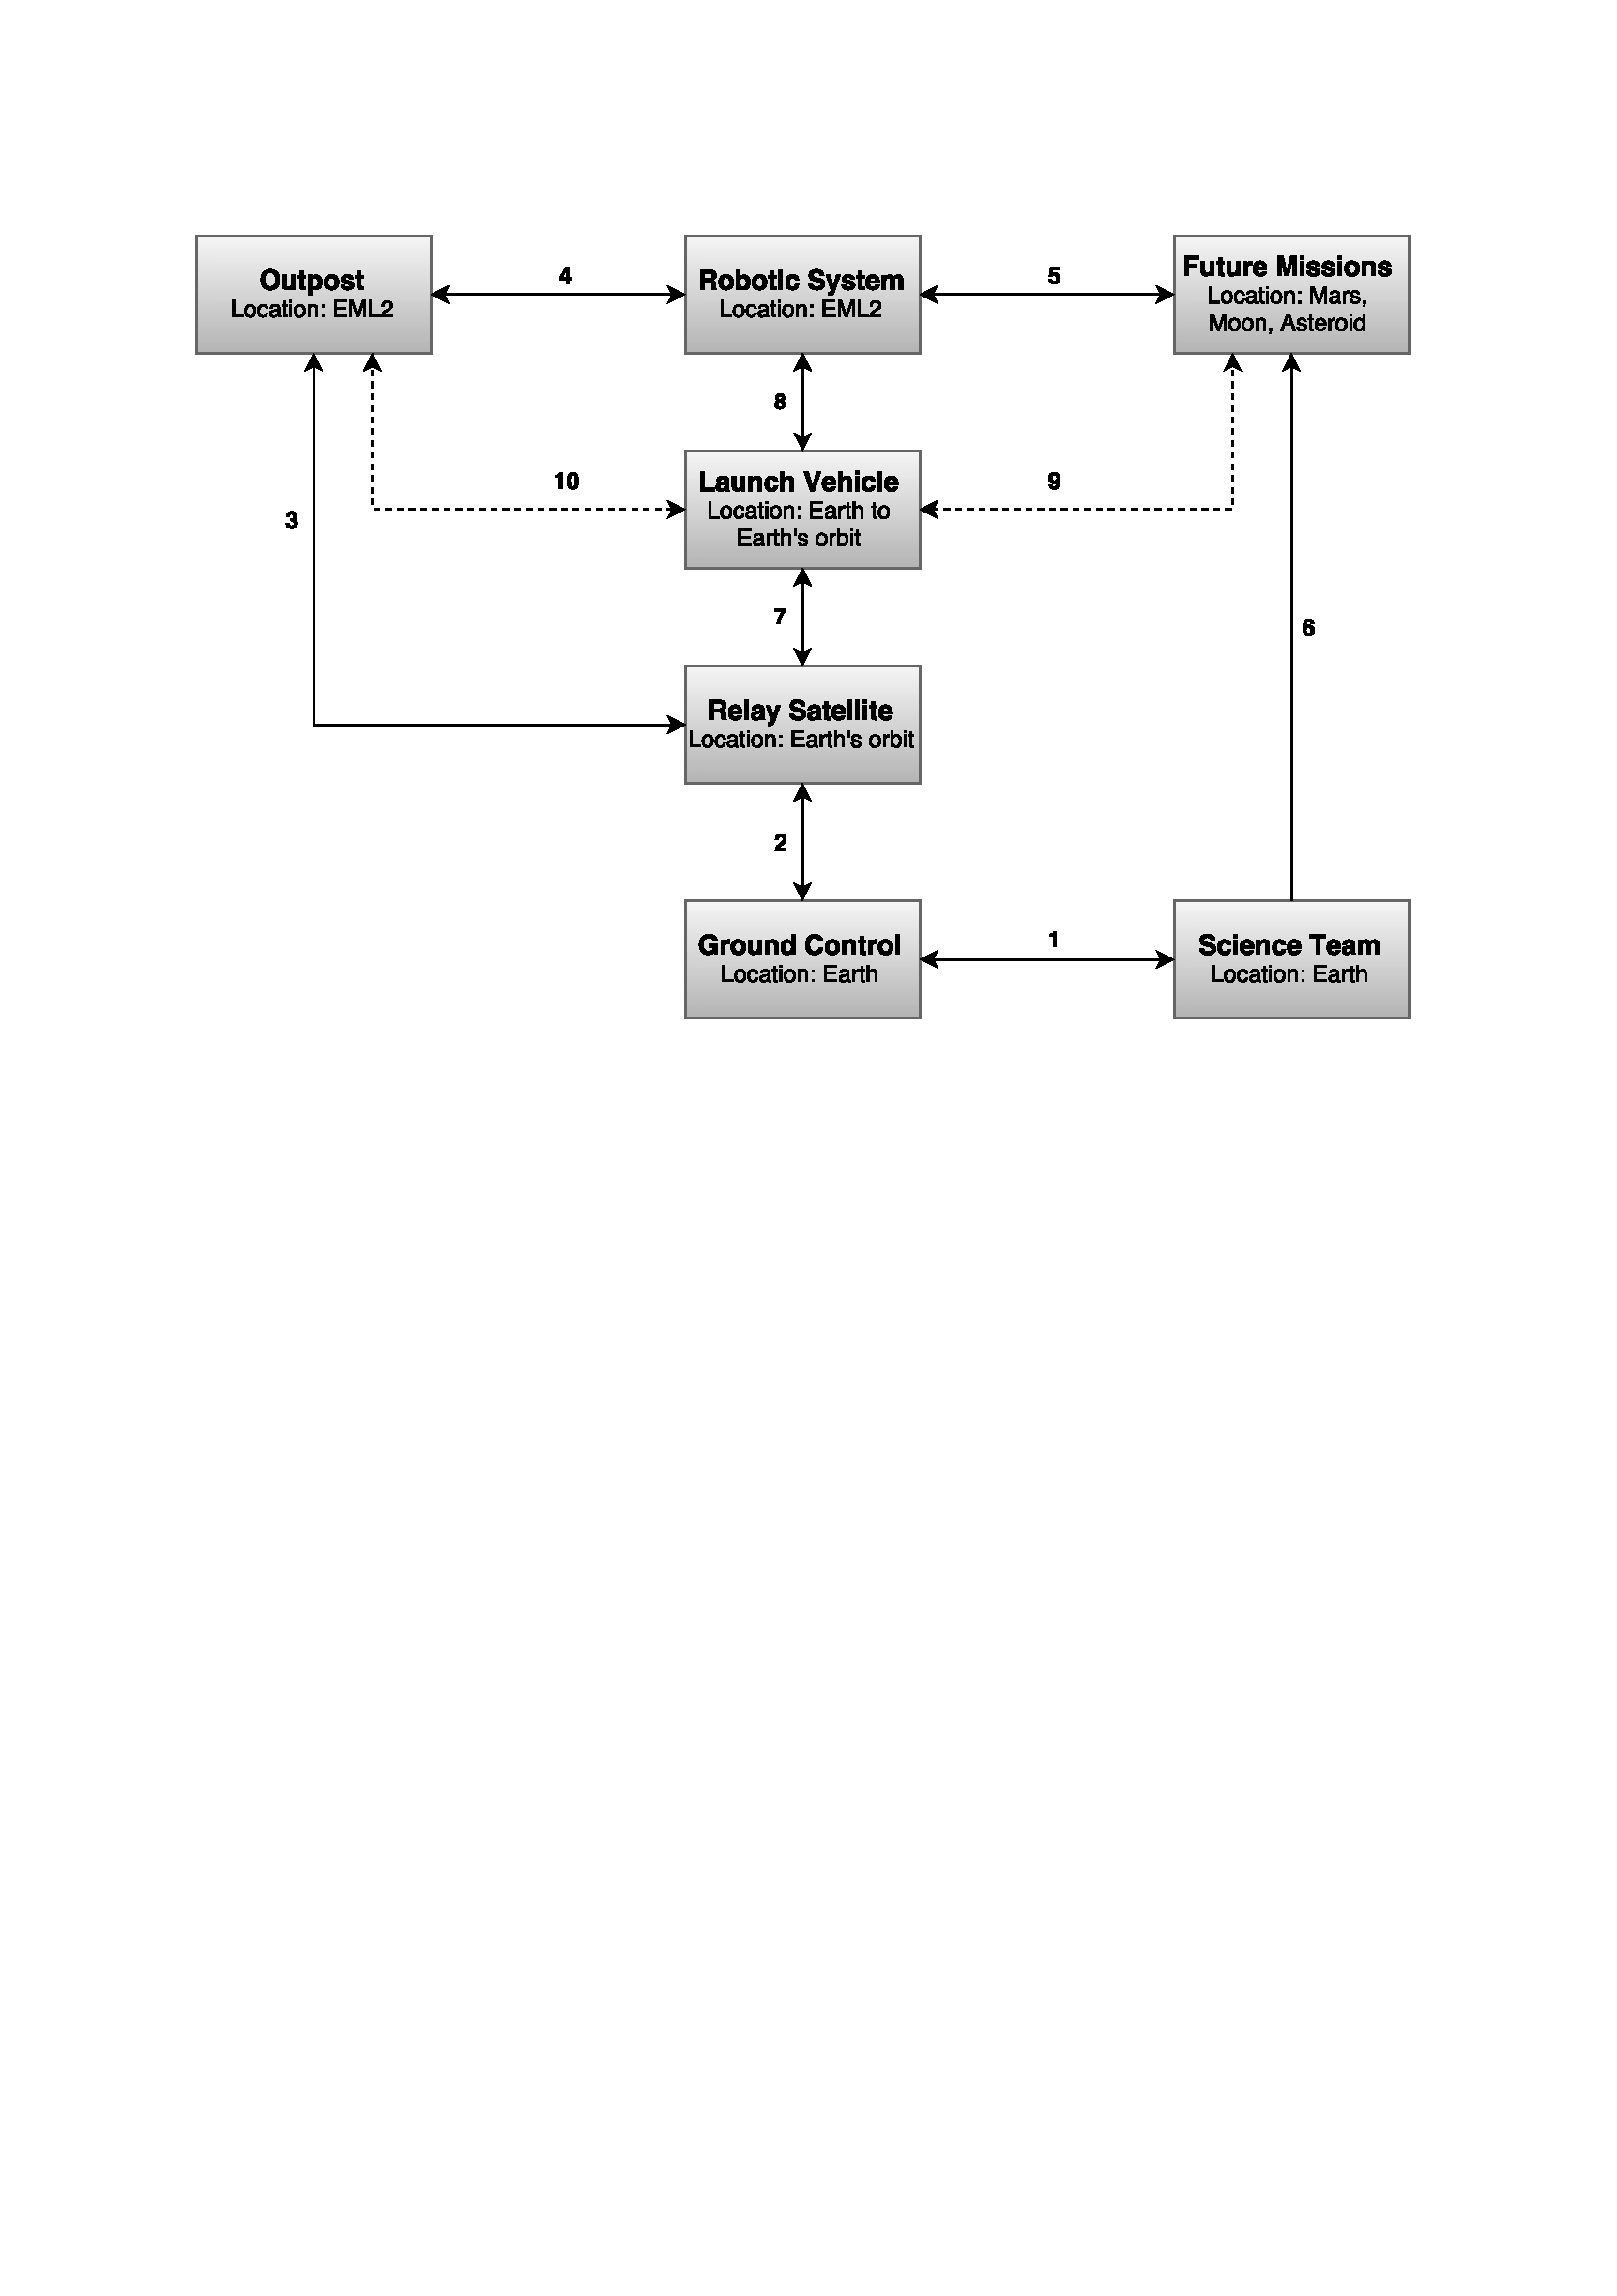
\includegraphics[width=0.9\textwidth]{missionlevel}
\caption{Mission-Level Block Diagram}
\end{figure}
\begin{enumerate}
\item{Science Team analyzes the Robotic System from a Science and Engineering perspective, and gives instruction to Ground Control based on desired operations. Ground Control relays information received to the Science Team.}
\item{Ground Control sends commands to, and receives information from the Outpost and Launch Vehicle through Relay Satellite.}
\item{Relay Satellite transfers signals between Ground Control and the Outpost.}
\item{The Outpost receives information from the Robotic System, and relays the information to Ground Control. The Outpost crew can directly control the Robotic System. In addition, the Robotic System is mechanically and electrically connected to the Outpost.}
\item{The Robotic System will be able to support future missions including ARM, and human-robotic missions on the surfaces of Mars and/or the Moon.}
\item{The Science Team will be responsible for organizing future missions involving asteroids, Mars, or the Moon. These missions are likely to use the Outpost.}
\item{The Relay Satellite transfers signals between Ground Control and Launch Vehicle.}
\item{Launch Vehicle provides the means for Robotic System to deploy into space, onto the Outpost. There is also an electromechanical interface between the two components.}
\item{Launch Vehicle may also carry payload for future missions to Mars, Moon, or Asteroids. However, this is not a direct part of the mission.}
\item{Launch Vehicle may also carry payload for other Outpost modules. However, this is not a direct part of the mission.}
\end{enumerate}

%--------------------------------------------------------------------------------------------------------------------------------------------------------------------------------
\section{Operational Scenarios}
\label{scenarios}
\vspace{-12pt}
\begin{figure}[H]
\centering
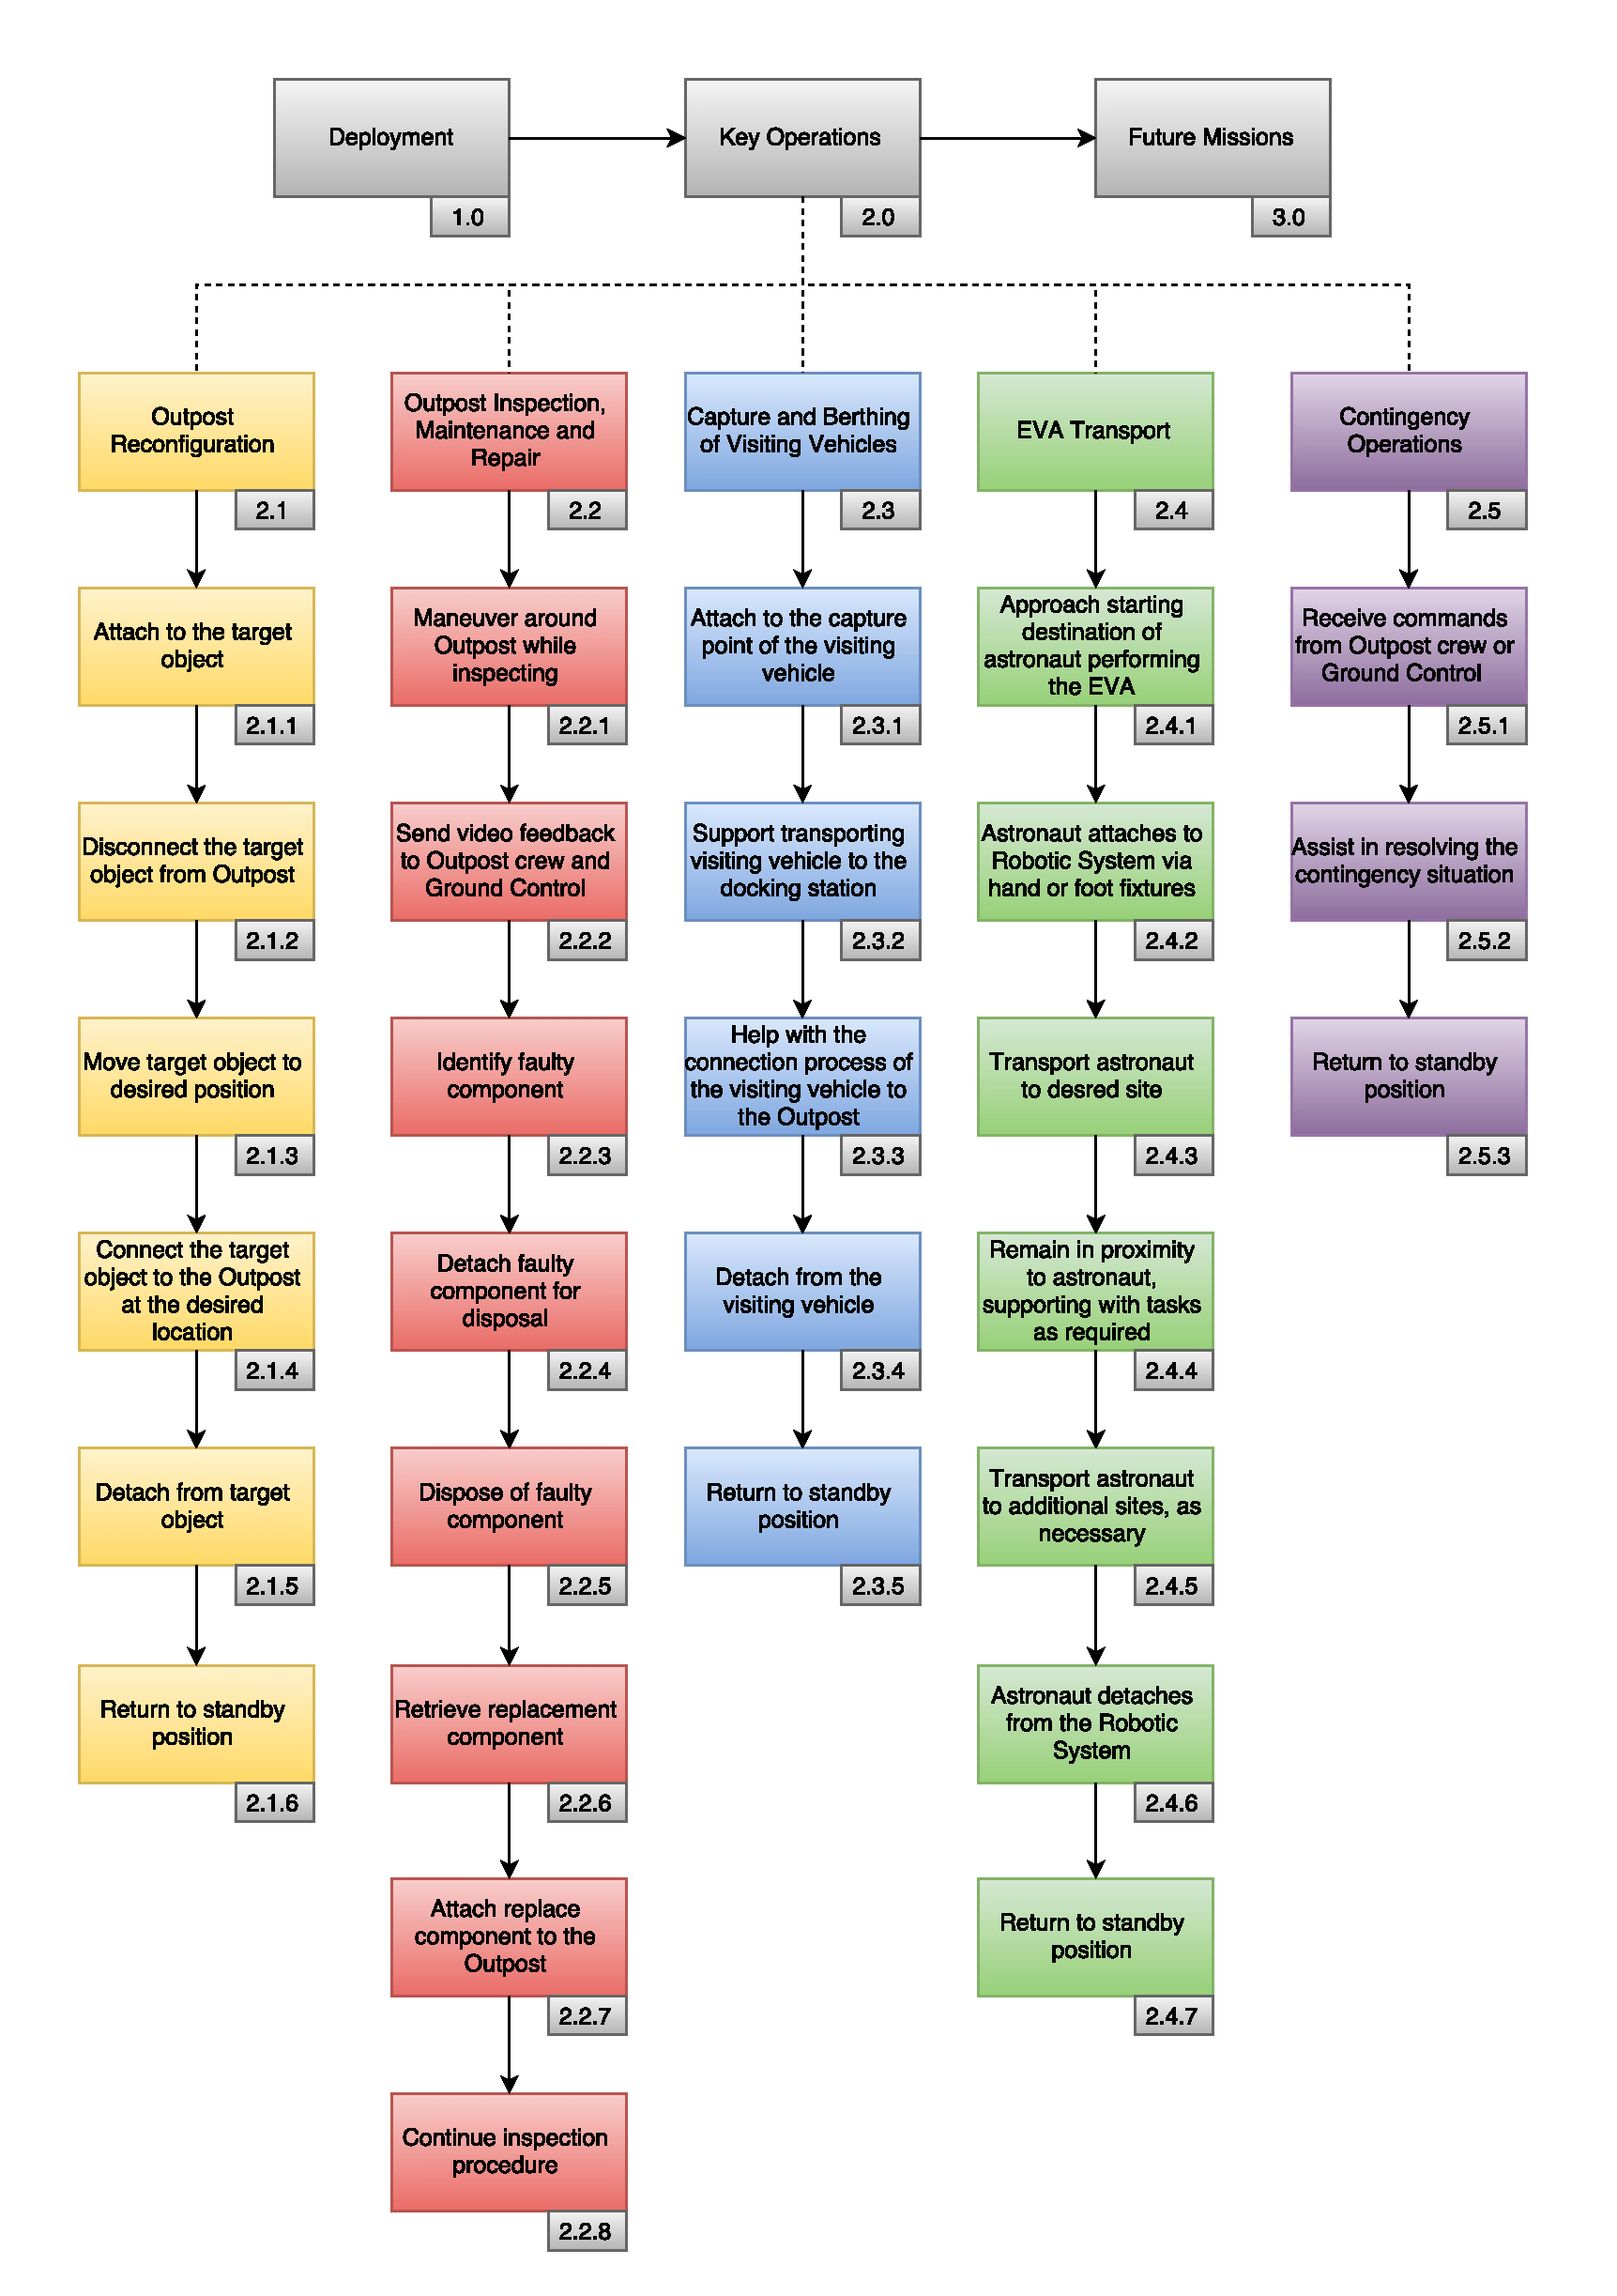
\includegraphics[height=0.95\textheight]{functionalflow}
\caption{Functional Flow Block Diagram (FFBD) describing the Top Level of Operations}
\label{FFBD}
\end{figure}
\begin{figure}[H]
\centering
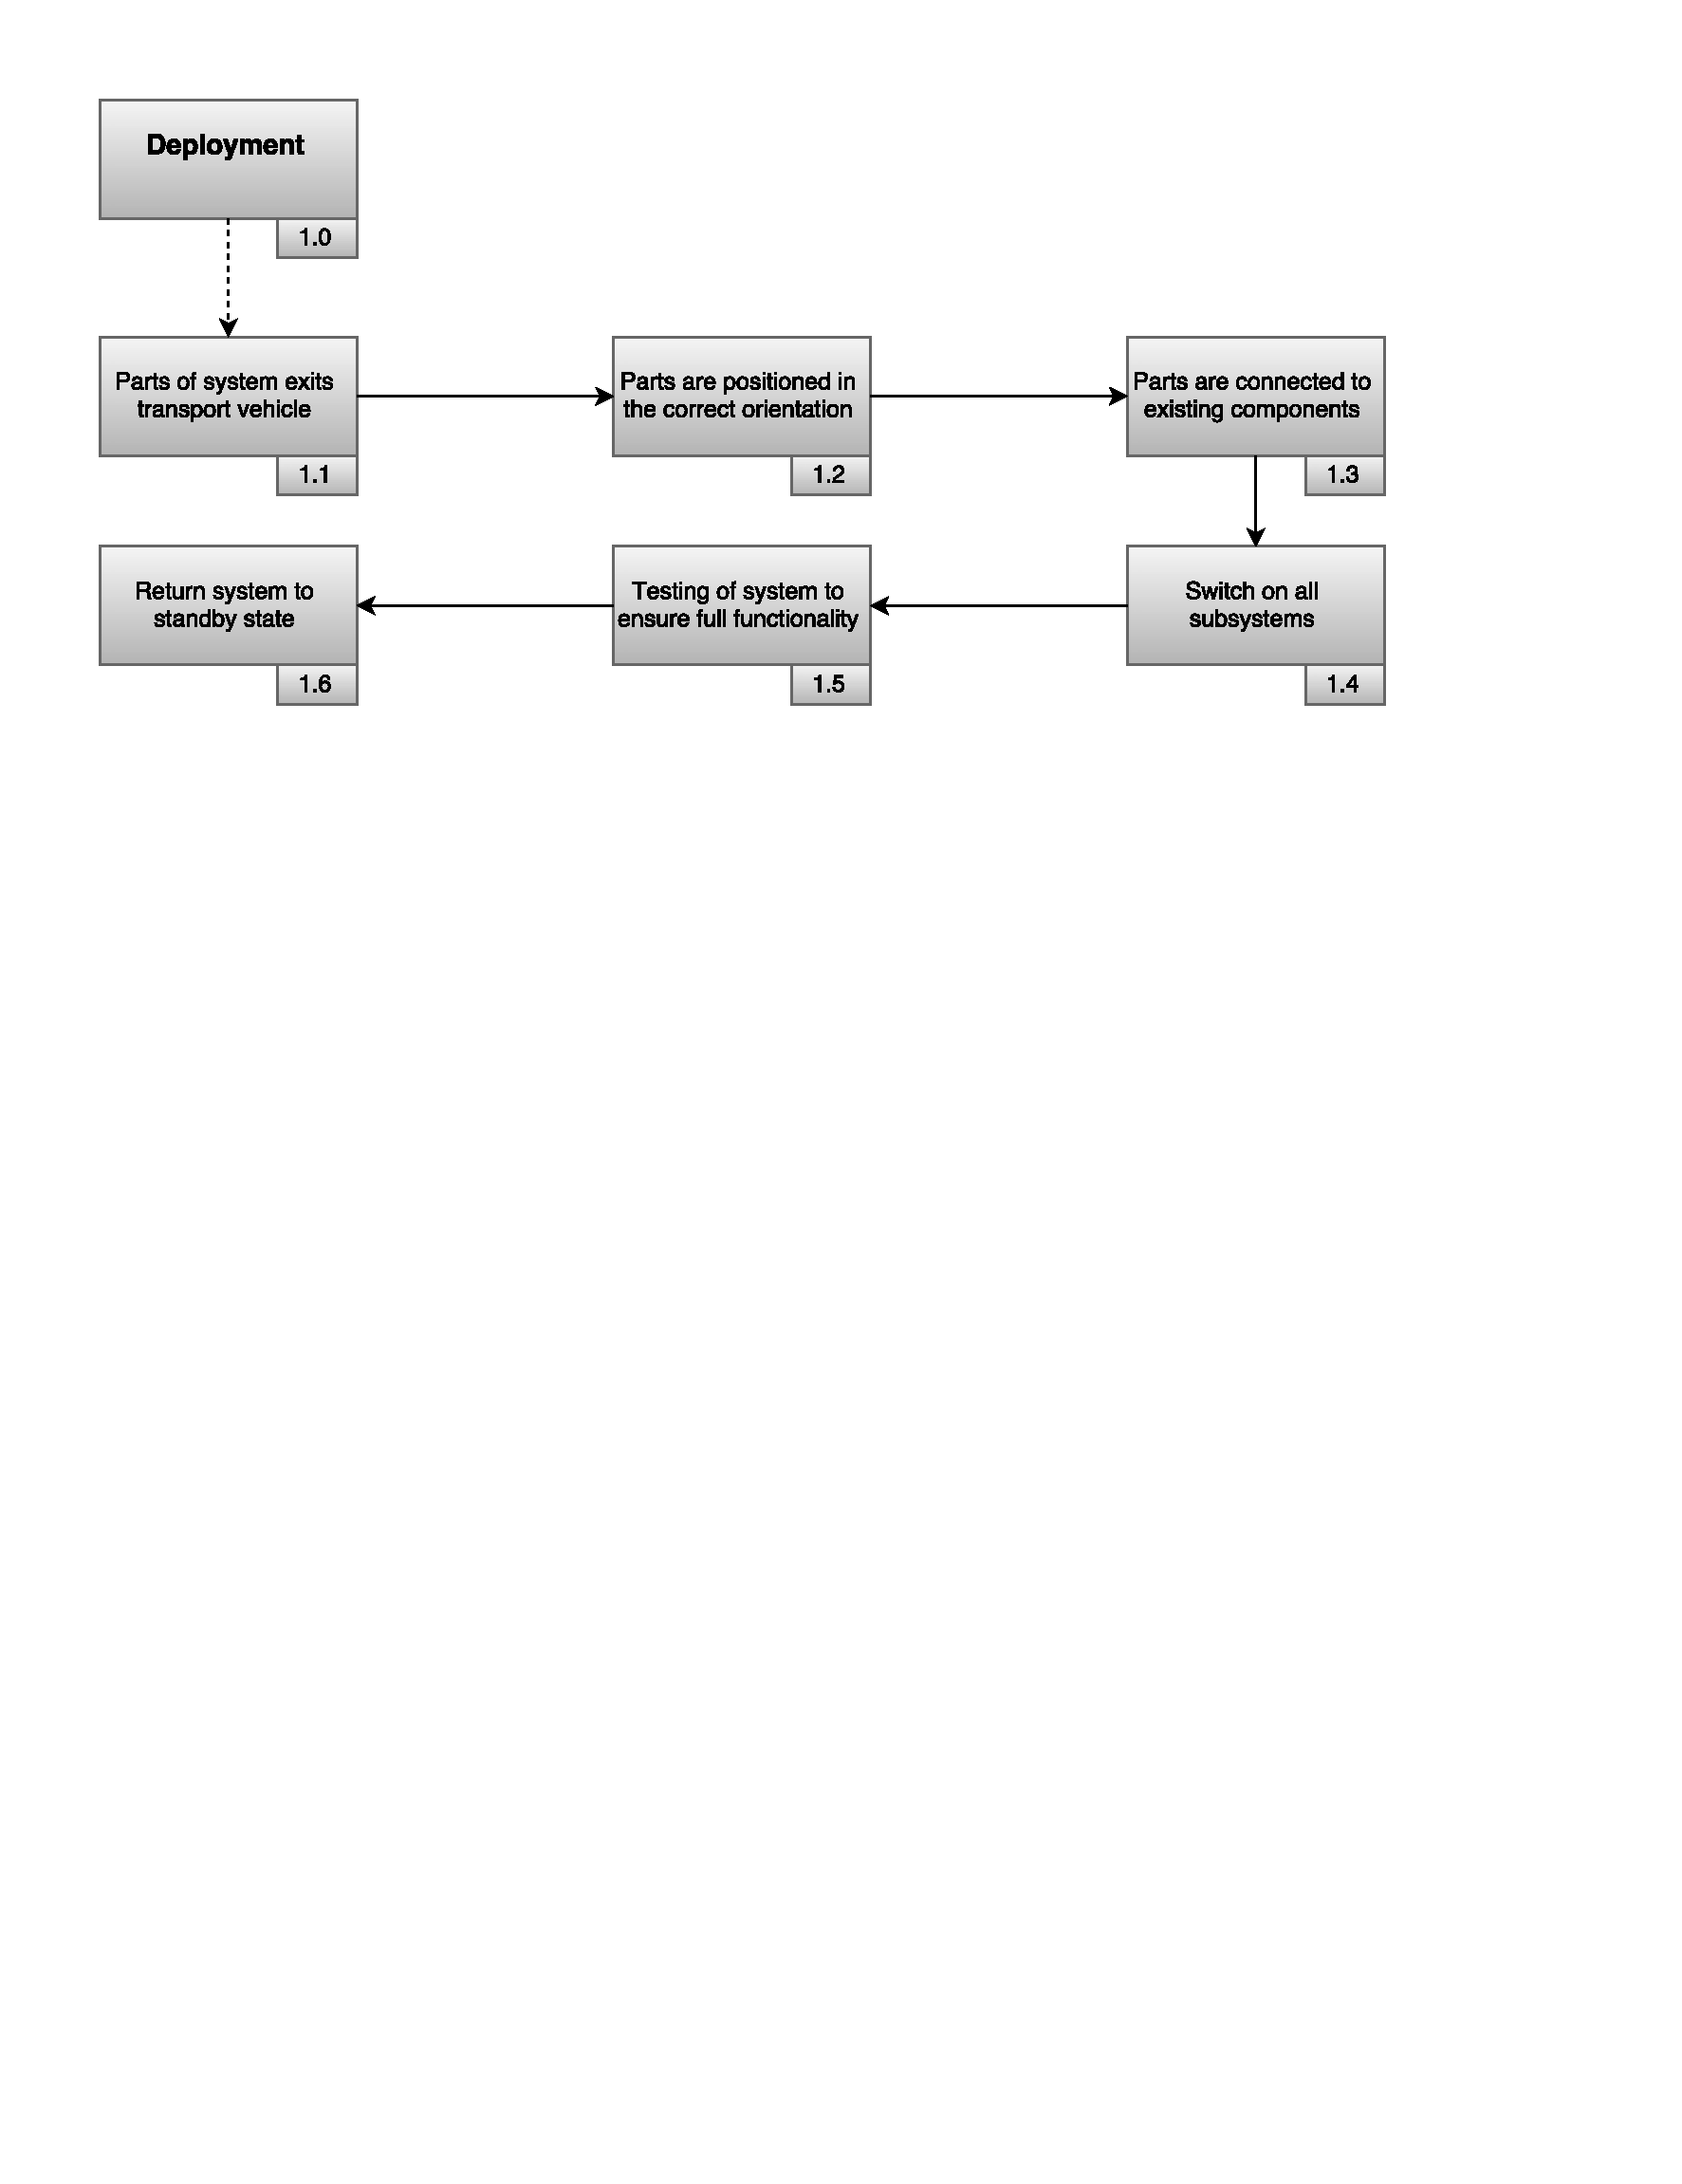
\includegraphics[width=0.9\textwidth]{deployment}
\caption{FFBD describing the First Level of Deployment Operations}
\label{deploy}
\end{figure}

\textbf{Deployment (1.0)}\\
The system will be launched in 6 stages, as shown in \Cref{deploy}. The parts will be removed from transport vehicle and positioned in the correct orientation. They are then connected to each other and tested for functionality before being returned to standby state to await instructions.\\

\textbf{Key Operations (2.0)}\\
The system has five key operations, as discussed in \Cref{goals} and shown in \Cref{FFBD}. Each of these operations are independent, and will be explained below.

\textbf{Outpost Reconfiguration (2.1)}\\
There are five general stages involved in this specific operation. First the target object is identified and attached to the system according to the command signal from the Outpost. Next the system will assist the target object to detach from the Outpost and be transported to its new position. The connection process at the new location will be supported by the system, before it detaches from the target object. Finally, the system will return to its standby state.

\textbf{Outpost Inspection, Maintenance and Repair (2.2)}\\
The system will be performing this function for a majority of the time on the Outpost. It will constantly maneuver around the Outpost, inspecting the various components of the individual modules while sending continuous video feedback to the Outpost crew and ground control. These user classes will be able to identify any faulty components either through inspection, or through the data received from these components. Once a faulty component is identified, the system will receive commands to detach the component through a standard procedure. In special cases, manual control can be used to carry out this procedure. Once the faulty component is disposed of, the system will retrieve the replacement component, and install it. Afterwards, the system will continue its inspection procedures.

\textbf{Capture and Berthing of Visiting Vehicles (2.3)}\\
This operation is similar to the reconfiguration explained in 2.2. First the system will carefully approach the visiting vehicle and attach to the designated capture point. The system will then help transfer the visiting vehicle to its docking location. Next the system will assist with the connection process,  and help adjust the visiting vehicle to the proper orientation and position. Once the vehicle has been properly docked to the Outpost, the system will detach itself and return to its standby state.

\textbf{EVA Transport (2.4)}\\
This operation will begin with the system approaching the starting destination of astronaut performing the EVA. The astronaut will then attach to the system (via hand or foot fixtures, tethers, etc.). The system will help transport the attached astronaut to the desired location, where it will remain in proximity to the astronaut, supporting with tasks as required. Next the system will transport the astronaut to additional sites, as necessary
until the EVA operation has been completed. Finally, the system will wait for the astronaut to detach before returning back to the standby state.

\textbf{Contingency Operations (2.5)}\\
The scenario of contingency operations largely depends on the specific situation of the contingency, therefore only a brief functional flow block diagram is provided for this operation. Some general steps include receiving commands from the Outpost crew or Ground Control based on the situation. Assisting in resolving the contingency situation according to the commands and returning to the standby state after the issue has been resolved.\\

\textbf{Future Missions (3.0)}\\
The system could also be customized to fit requirements of future missions. Below are three examples of potential future missions and how the system can be customized to perform such missions.
\begin{itemize}
\item{\textbf{Asteroid Capture}: System could be mounted onto another spacecraft and fitted with additional mechanisms to locate and capture asteroids}
\item{\textbf{Lunar Surface}: System could be relocated to lunar surface by another spacecraft to support logistics handling on Moon}
\item{\textbf{Mars Surface}: System could be relocated to Mars surface to assist in construction of Mars Outpost and possibly capture of incoming spacecraft for safe landings}
\end{itemize}


\newpage
\bibliographystyle{unsrt}
\bibliography{reportbib}

\newpage
\appendix
\section{Correspondence}
\label{email}
\begin{figure}[H]
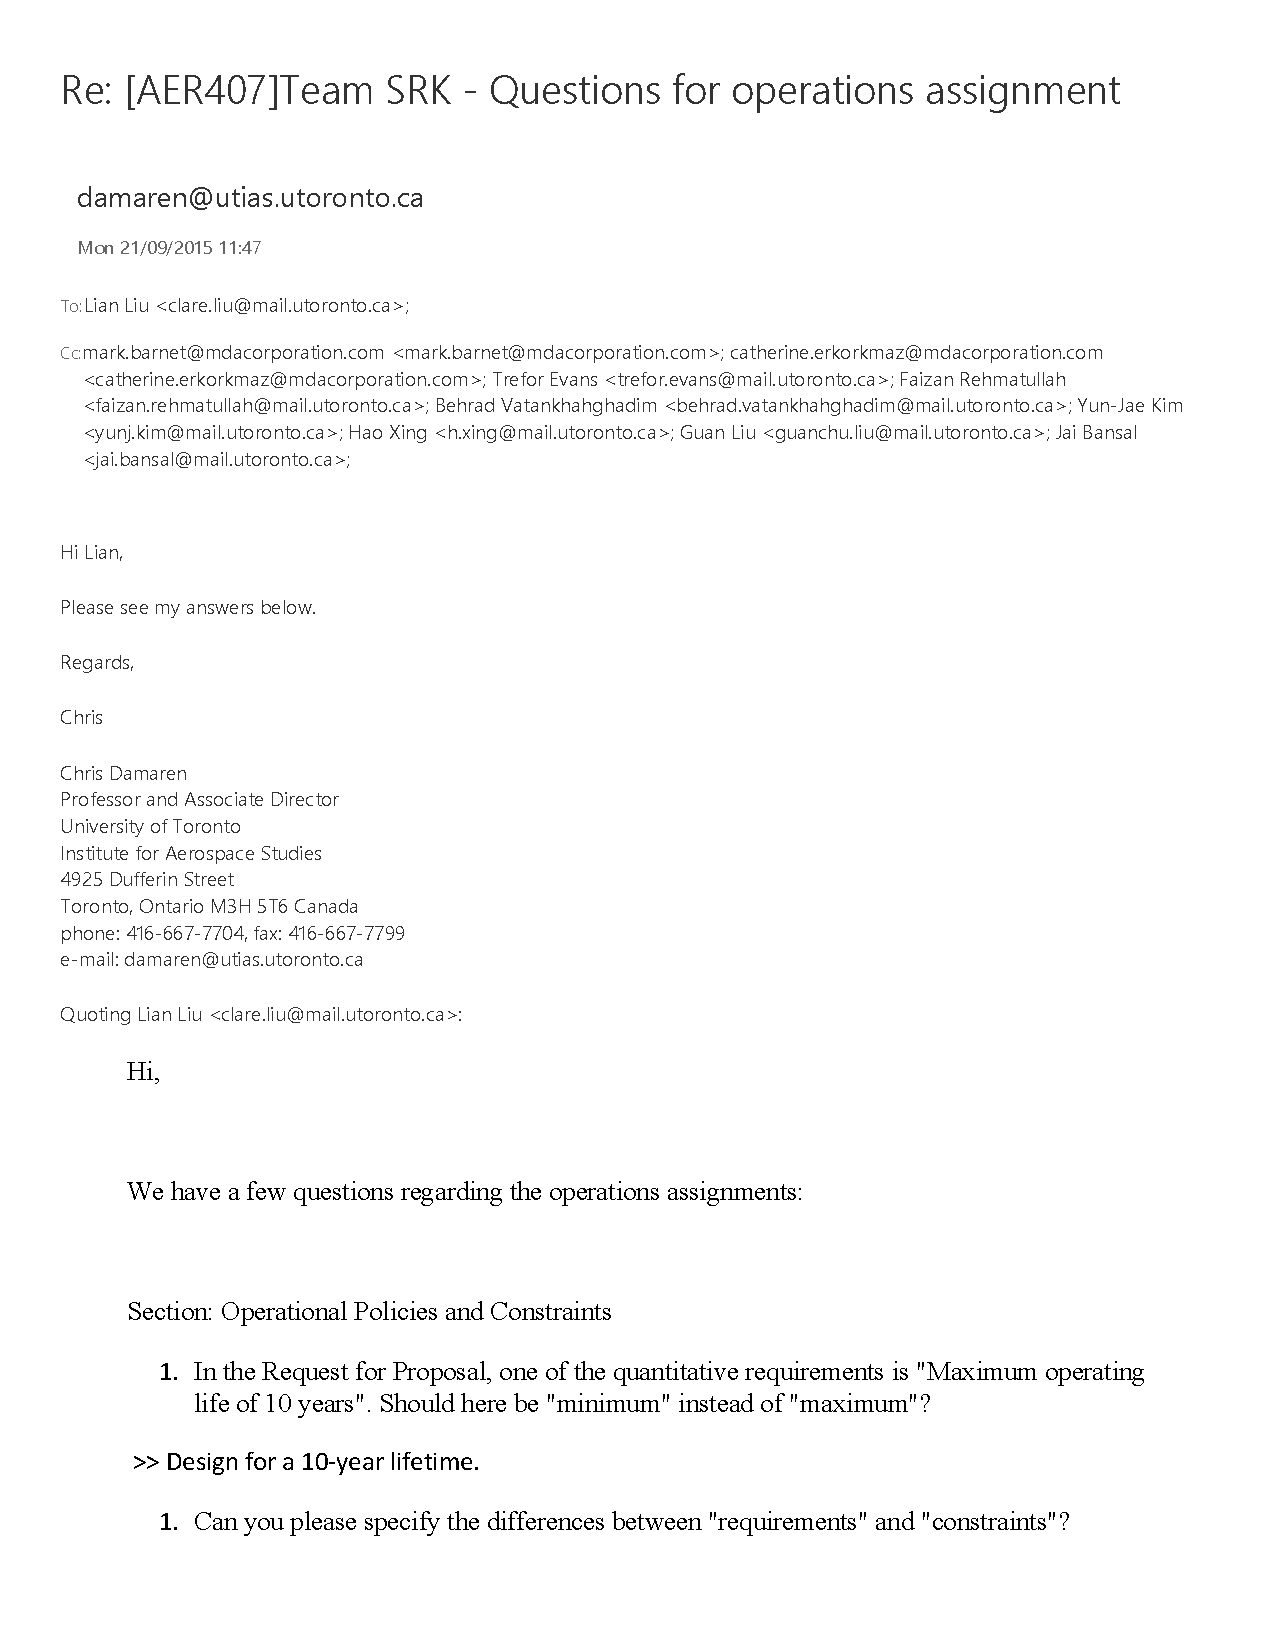
\includegraphics[height=\textheight]{email}
\end{figure}
\begin{figure}[H]
\includegraphics[height=\textheight, page=2]{email}
\end{figure}

\newpage
\section{Allowable Volumes}
\label{volumes}
\begin{table}[H]
\caption{Volumes of Transport Vehicles that can be used\cite{RFP}}
\centering
\begin{tabular}{|c|c|c|}
\hline
\textbf{Launch Vehicle}	&	\textbf{Detailed Volume}				&	\textbf(Dimensions)	\\
				&										&	(Length $\times$ Width $\times$ Height)	\\\hhline{|=|=|=|}
\textbf{ARV}		&	\begin{minipage}{5.5cm}
					\centering
					\vspace{2px}
					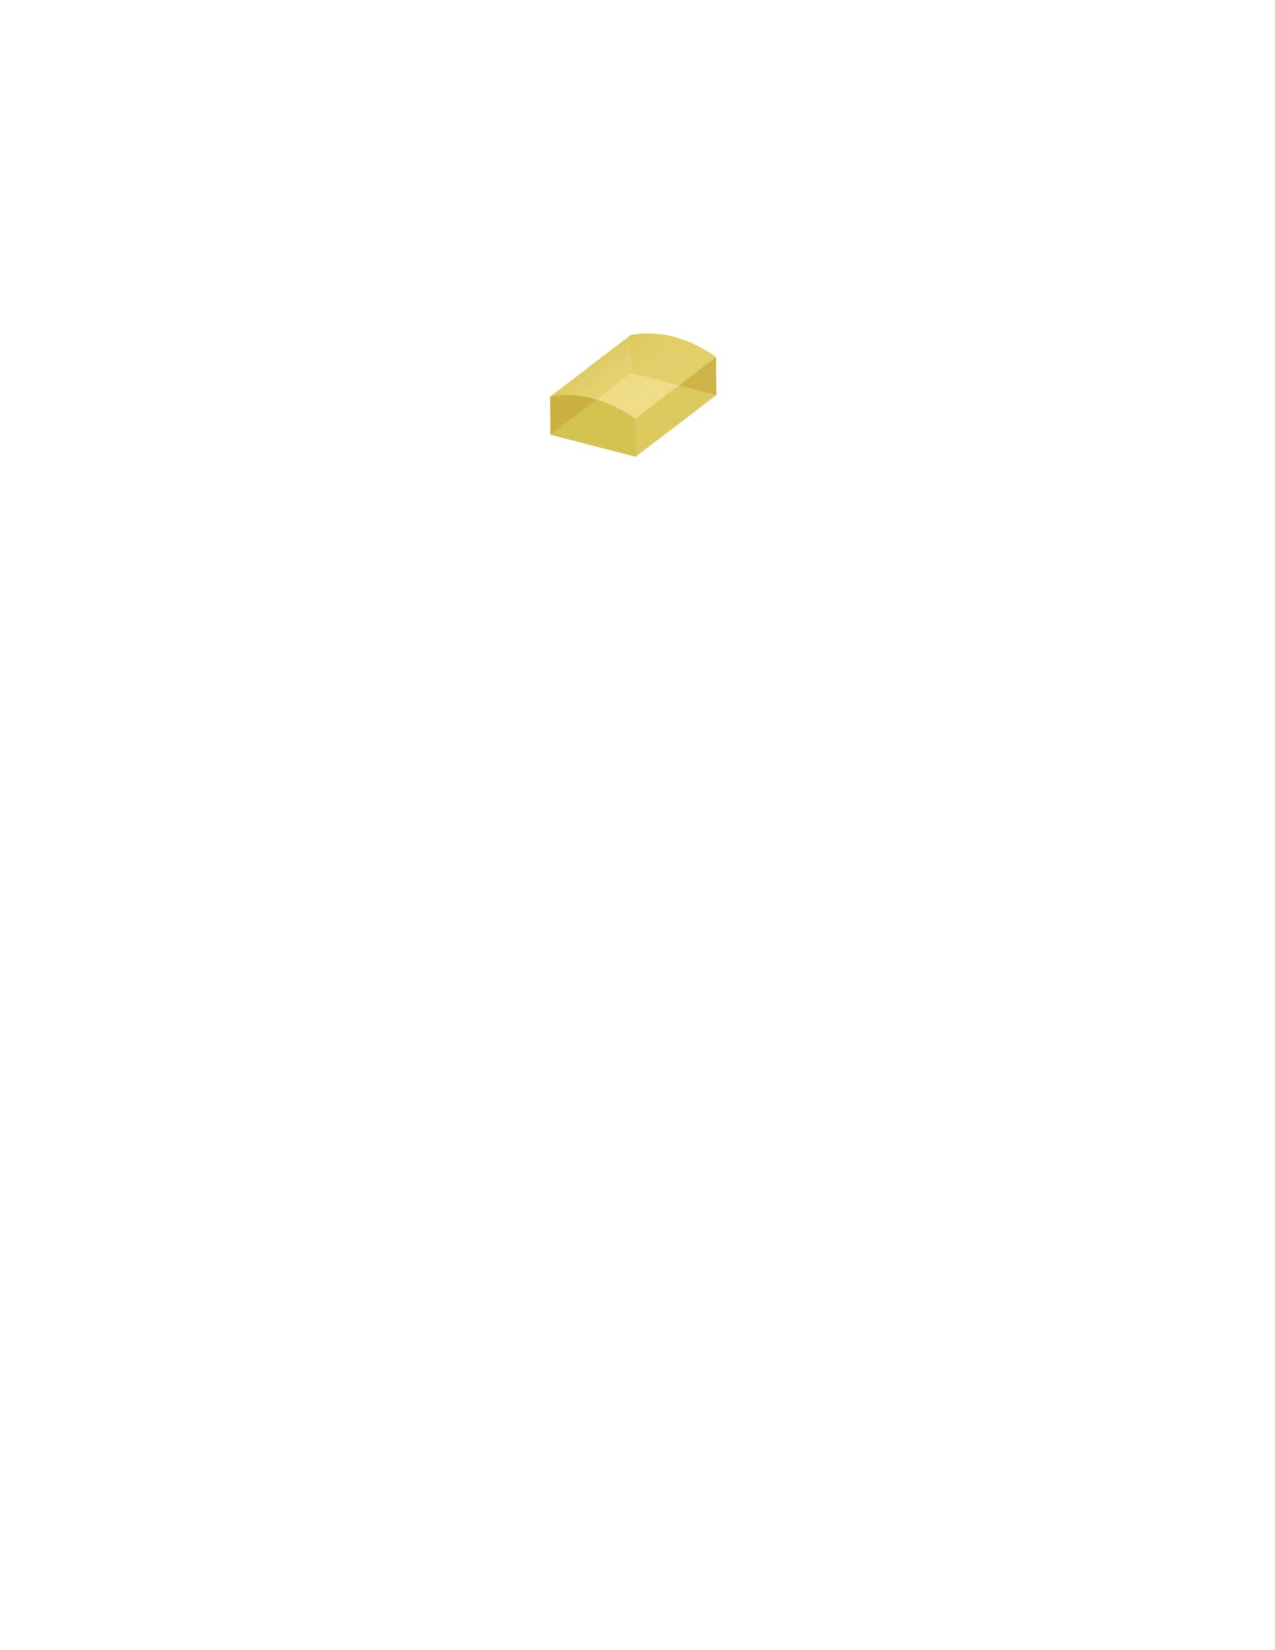
\includegraphics[width=3.5cm]{ARV_step}	
					\end{minipage}							&	\SI{3.8}{\m} $\times$ \SI{1.8}{\m} $\times$ \SI{0.67}{\m}	\\\hline
\textbf{Orion MPCV}	&	\begin{minipage}{5.5cm}
					\centering
					\vspace{2px}
					
\includegraphics[width=5cm]{MPCV_step}	
					\end{minipage}							&	\SI{4.0}{\m} $\times$ \SI{1.3}{\m} $\times$ \SI{0.58}{\m}	\\\hline
\end{tabular}
\end{table}

\end{document}
